\documentclass{article}

\usepackage{url}
\usepackage{fancyhdr}
\usepackage{extramarks}
\usepackage{amsmath}
\usepackage{amsthm}
\usepackage{amsfonts}
\usepackage{tikz}
\usetikzlibrary{3d}
\usepackage[plain]{algorithm}
\usepackage{algpseudocode}
\usepackage{braket}
\usepackage{enumerate}
\usepackage{paralist}

%
% Basic Document Settings
%

\topmargin=-0.45in
\evensidemargin=0in
\oddsidemargin=0in
\textwidth=6.5in
\textheight=9.0in
\headsep=0.25in

\linespread{1.1}

\pagestyle{fancy}
\lhead{Habib University}
\chead{\hmwkClass, \hmwkTitle}
\rhead{\firstxmark}
\lfoot{\lastxmark}
\cfoot{\thepage}

\renewcommand\headrulewidth{0.4pt}
\renewcommand\footrulewidth{0.4pt}

\setlength\parindent{0pt}

%
% Create Problem Sections
%

\newcommand{\enterProblemHeader}[1]{
	\nobreak\extramarks{}{Problem \arabic{#1} continued on next page\ldots}\nobreak{}
	\nobreak\extramarks{Problem \arabic{#1} (continued)}{Problem \arabic{#1} continued on next page\ldots}\nobreak{}
}

\newcommand{\exitProblemHeader}[1]{
	\nobreak\extramarks{Problem \arabic{#1} (continued)}{Problem \arabic{#1} continued on next page\ldots}\nobreak{}
	\stepcounter{#1}
	\nobreak\extramarks{Problem \arabic{#1}}{}\nobreak{}
}

\setcounter{secnumdepth}{0}
\newcounter{partCounter}
\newcounter{homeworkProblemCounter}
\setcounter{homeworkProblemCounter}{1}
\nobreak\extramarks{Problem \arabic{homeworkProblemCounter}}{}\nobreak{}

%
% Homework Problem Environment
%
% This environment takes an optional argument. When given, it will adjust the
% problem counter. This is useful for when the problems given for your
% assignment aren't sequential. See the last 3 problems of this template for an
% example.
%
\newenvironment{homeworkProblem}[1][-1]{
	\ifnum#1>0
	\setcounter{homeworkProblemCounter}{#1}
	\fi
	\section{Problem \arabic{homeworkProblemCounter}}
	\setcounter{partCounter}{1}
	\enterProblemHeader{homeworkProblemCounter}
}{
	\exitProblemHeader{homeworkProblemCounter}
}

%
% Homework Details
%   - Title
%   - Due date
%   - Class
%   - Section/Time
%   - Instructor
%   - Author
%

\newcommand{\hmwkTitle}{Assignment\ \#1}
\newcommand{\hmwkDueDate}{February 10, 2024, 11.59pm}
\newcommand{\hmwkClass}{CS 201 - Data Structures and Algorithms II}
\newcommand{\hmwkClassInstructor}{Muhammad Mobeen Movania (L1),\\ Syeda Saleha Raza (L2),\\ Faisal Alvi (L3, L4),\\ Abdullah Zafar (L5).}
\newcommand{\hmwkAuthorName}{\textbf{Student 1 Name, ID} \and \textbf{Student 2 Name, ID}}

%
% Title Page
%

\title{
	\vspace{2in}
	\textmd{\textbf{\hmwkClass:\\ \hmwkTitle}}\\
	\normalsize\vspace{0.1in}\small{\hmwkClassInstructor}\\
	\normalsize\vspace{0.1in}\small{Due\ on\ \hmwkDueDate}\\
	\vspace{3in}
}

\author{\hmwkAuthorName}
\date{}

\renewcommand{\part}[1]{\textbf{\large Part \Alph{partCounter}}\stepcounter{partCounter}\\}

%
% Various Helper Commands
%

% Useful for algorithms
\newcommand{\alg}[1]{\textsc{\bfseries \footnotesize #1}}

% For derivatives
\newcommand{\deriv}[1]{\frac{\mathrm{d}}{\mathrm{d}x} (#1)}

% For partial derivatives
\newcommand{\pderiv}[2]{\frac{\partial}{\partial #1} (#2)}

% Integral dx
\newcommand{\dx}{\mathrm{d}x}

% Alias for the Solution section header
\newcommand{\solution}{\textbf{\large Solution}}

% Probability commands: Expectation, Variance, Covariance, Bias
\newcommand{\E}{\mathrm{E}}
\newcommand{\Var}{\mathrm{Var}}
\newcommand{\Cov}{\mathrm{Cov}}
\newcommand{\Bias}{\mathrm{Bias}}

\begin{document}
	
\maketitle
	
\pagebreak
\section{Instructions}
This assignment document consists of two problems.

\begin{itemize} 
	\item \underline{Problem 1} is a theoretical question which requires analysis. It should be completed and submitted within this document. This problem is worth 20 points.
	\item \underline{Problem 2} is a programming based question which requires implementation. It must be submitted as a zipped archive containing:
\begin{enumerate}
	\item your programs (the language of implementation in C++), 
	\item the input files provided to you, and
	\item the output files generated by your program. 
\end{enumerate}

The solution to program 2 will be graded for correctness and structure by testing the output against test input files. This problem is worth 40 points.

\end{itemize}
\newpage
\begin{homeworkProblem}
(20 points) [\textbf{Amortized Analysis}] Let us define a \texttt{stop-min-stack} with a stack as the underlying data structure, which stores a sequence of items and has the following operations:
\begin{enumerate}
	\item \texttt{push(\textit{x})} adds the item \texttt{\textit{x}} to the top of the underlying stack.
	\item \texttt{peek()} returns the item at the top of the underlying stack without removing it.
	\item \texttt{stop-min-pop()} pops a local minimum from the existing items in the stack. This operation works as follows:
	\begin{enumerate}[(a)]
		\item removes an existing item from the stack using \texttt{pop()}, (if the stack was empty before the \texttt{pop()}, NULL is returned; if the stack is empty as a result of the \texttt{pop()}, the popped item is returned) 
		\item tests whether the popped item is greater than or equal to the current item at the top of the underlying stack using \texttt{peek()}. 
		\item If yes, the recently popped item is discarded. 
		\item Steps (a) - (c) are repeated as a loop until the recently popped item is less than the topmost item in the stack or if the underlying stack is empty. 
		\item Finally, the recently popped item is returned.
	\end{enumerate}
\end{enumerate}
For example if the stack contains the items 4, 3, 2, 9, 5, then after one application of \texttt{stop-min-pop()}, the item 2 will be returned and the stack will have the elements 9, 5 as shown below:
% Please add the following required packages to your document preamble:
% \usepackage{graphicx}

\begin{table}[h]
	\centering
	\begin{tabular}{|c|c|c|}
			4 &  &   \\ \cline{1-1}
			3 &  &   \\ \cline{1-1}
			2 &  &   \\ \cline{1-1} \cline{3-3} 
			9 &  & 9 \\ \cline{1-1} \cline{3-3} 
			5 &  & 5 \\ \cline{1-1} \cline{3-3} 
		\end{tabular}%
	\caption{\texttt{Stop-min-stack} before and after one application of \texttt{stop-min-pop()}}
\end{table}

%%\begin{figure} [H]
%% 	\centering
%% 	\includegraphics[scale = 0.7]{bell-states.png}
%% 	\caption{The Four Bell States $\ket{\phi^+}$, %%$\ket{\phi^-}$, $\ket{\psi^+}$, $\ket{\psi^-}$}
%%\end{figure}
		
\begin{enumerate}[(a)]
\item (5 points) Using an underlying Stack which has only \texttt{push}, \texttt{pop} and \texttt{peek} as its operations with constant time complexity, write pseudocode for the operation \texttt{stop-min-pop()}. What is the time complexity of \texttt{stop-min-pop()} in the worst case for a stack of size $n$? 
\item (5 points) Give an argument using worst case analysis that if \texttt{stop-min-pop()} is applied $n$ times to an arbitrary stack of size $n$, the worst case time complexity can be O$(n^2)$, thereby giving a cost of O$(n)$ per operation.

\item (10 points) Using amortized analysis, show that the amortized cost of applying \texttt{stop-min-pop()} $n$ times to an arbitrary stack of size $n$ is actually O(1) per operation.
\end{enumerate}

\end{homeworkProblem}
\bigskip

\newpage
\begin{homeworkProblem} (40 points) [\textbf{Simplifying Postscript files by evaluating stack based expressions}] 

Postscript is a programming language that has been widely used for publishing documents. It is a stack based language that can be used to construct very simple to complex graphics as well as text. Modern documents in PDF (portable document format) use postscript as part of the document structure for rendering graphics.
	
Some examples of postscript graphics are given below:
\begin{figure} [H]
	\centering
	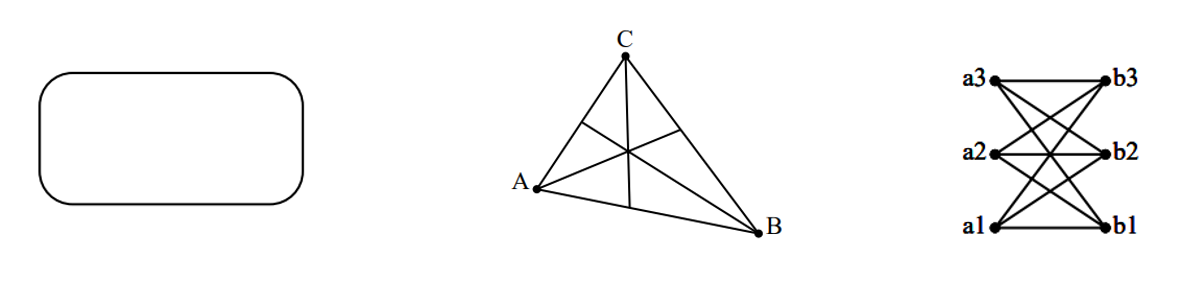
\includegraphics[scale = 0.5]{fig/ps-examples.png}
	\caption{Examples of Postscript Graphics}
\end{figure}

A postscript file (or encapsulated postscript file) has an extension .ps (or .eps) and can be opened and edited in a text editor. The drawing canvas has coordinates starting from (0, 0) at the bottom left corner of the page with coordinates increasing in the positive X and Y directions. As an example, the following postscript code on the left displays the image on the right.

\begin{figure} [H]
	\centering
	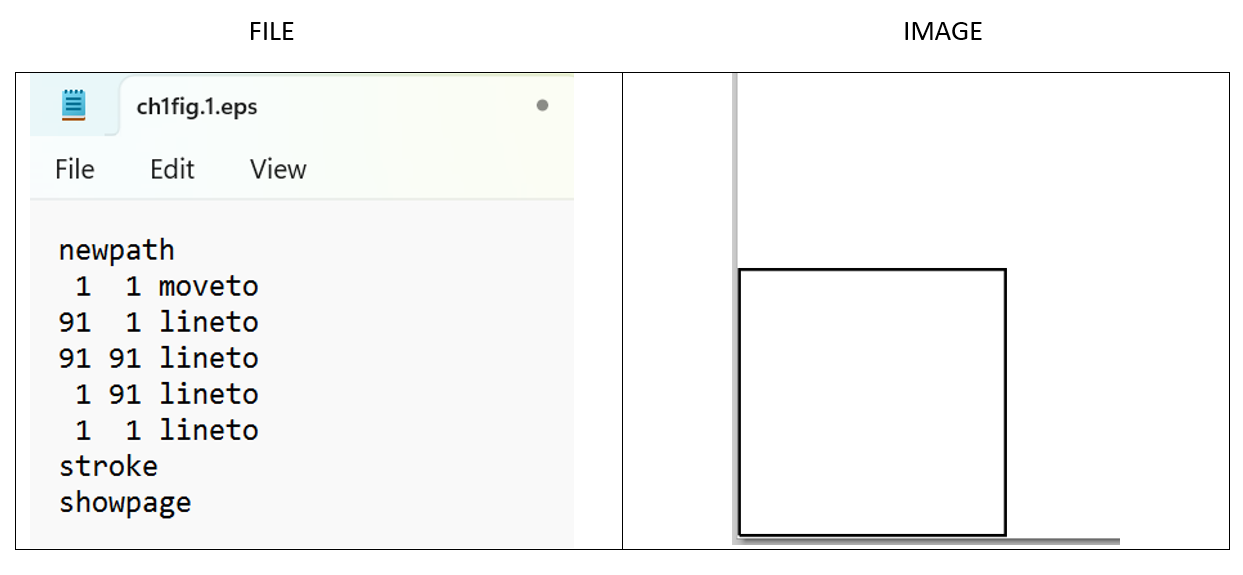
\includegraphics[scale = 0.5]{fig/ps-code-image-example.png}
	\caption{Postscript Code (Left) with Example (Right)}
\end{figure}

For a more complete reference to postscript you may consult the following tutorial: Learn Postscript by Doing (\url{ https://staff.science.uva.nl/a.j.p.heck/Courses/Mastercourse2005/tutorial.pdf}) 
\vspace{0.5cm}

To display a postscript file, several programs can be used both online as well as offline. We use Inkscape (\url{https://inkscape.org/}) a free and open source vector graphics software to render images in this document.

\textbf{Stacks:} Postscript uses a stack for all its computations including mathematical as well as stack based manipulation. A list of stack based operators for postscript are shown in the following tables:

\begin{figure} [H]
	\centering
	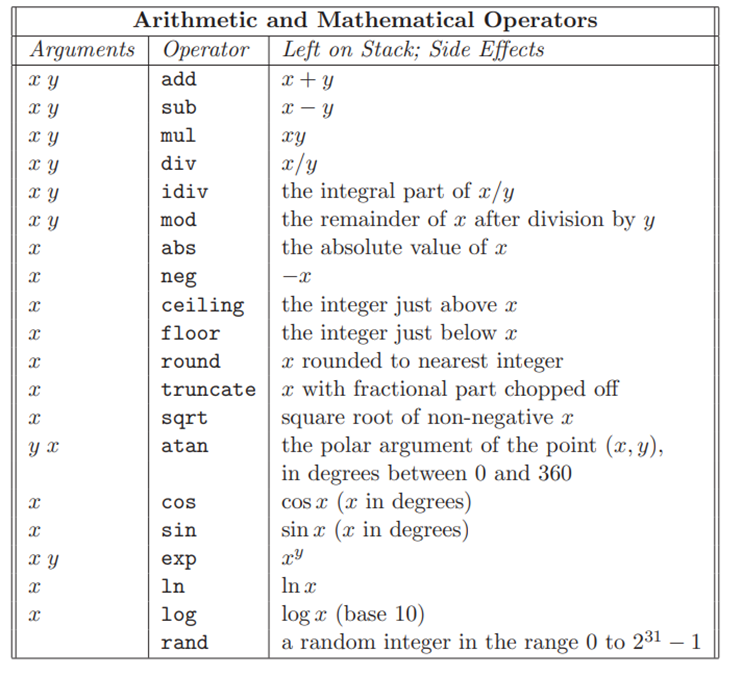
\includegraphics[scale=0.50]{fig/math-stack-operators.png}
	\caption{Arithmetic and Mathematical Operators}
\end{figure}

\begin{figure} [H]
	\centering
	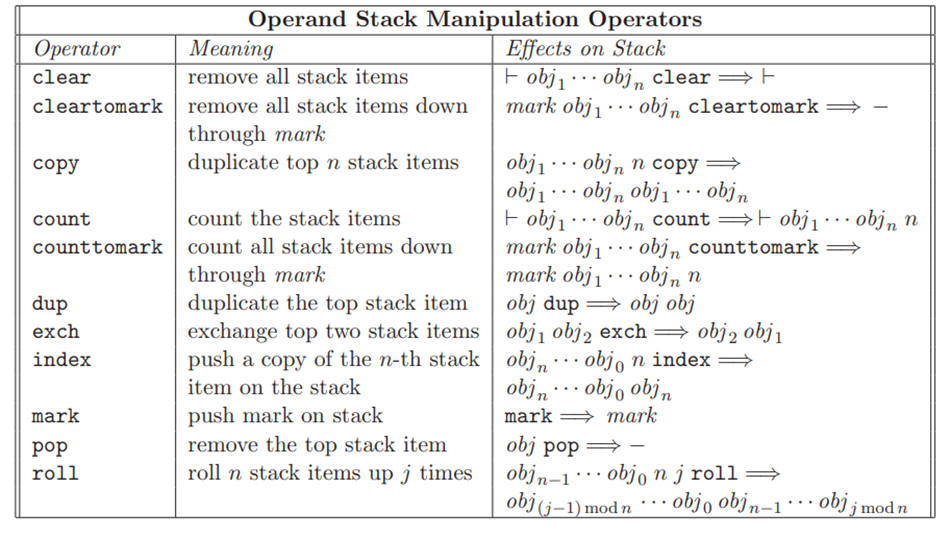
\includegraphics[scale=0.50]{fig/stack-manipulation-operators.png}
	\caption{Stack Manipulation Operators}
\end{figure}

For the purpose of this assignment, we will be using the following operators only: 

\vspace{0.5cm}

\texttt{add, sub, mul, div, sin, cos, mod, exp, sqrt, dup, exch, roll}. 

\vspace{0.5cm}

Additionally, you may use any other operators that may be required to implement the above list of operators.

\vspace{0.5cm}

\textbf{Variable or Procedure Declaration:} You can declare a variable (or a procedure) in postscript using a ``/'' preceding the variable (or procedure) name, followed by the variable (or procedure) definition, and ending with a ``def'' as shown in the following figure:

\begin{figure} [H]
	\centering
	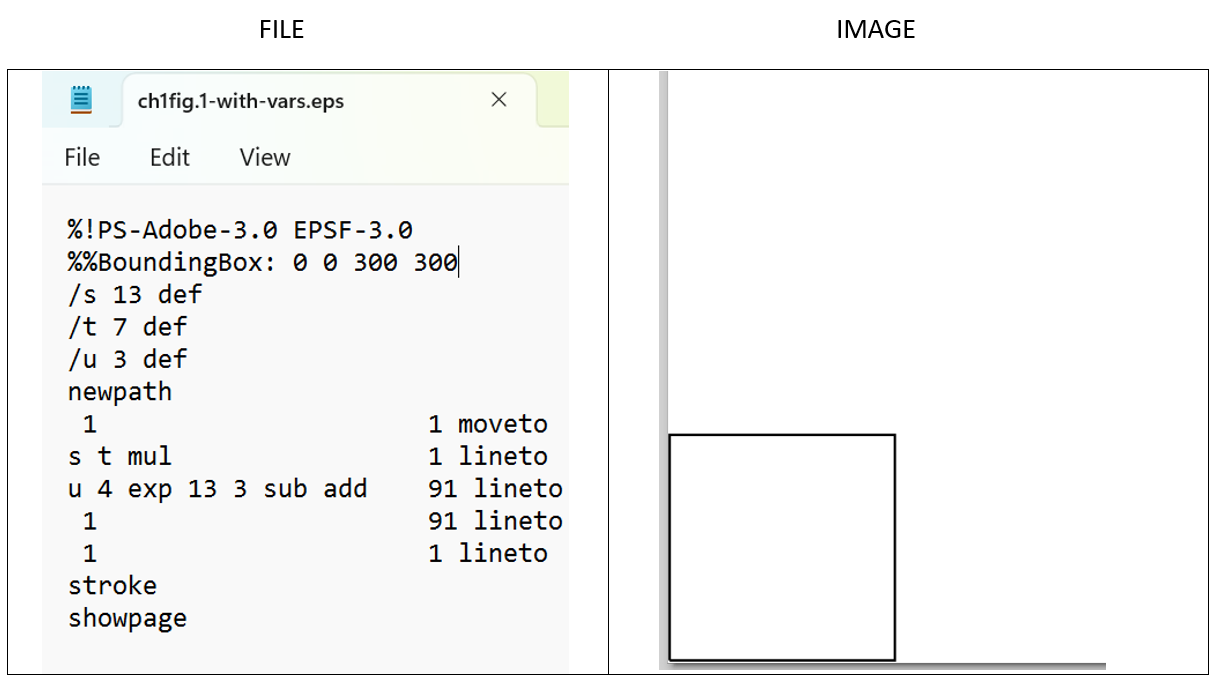
\includegraphics[scale=0.45]{fig/varOrProcDeclarations.png}
	\caption{Variable Declarations: s, t and u are variables}
\end{figure}

Note that this file renders the same square as the previous example. However, here we declare three variables s, t and u. Furthermore,
\begin{itemize}
\item \texttt{s t mul} evaluates to \texttt{13 7 mul} on the stack $\Rightarrow$ 13 $\cdot$ 7 = 91
\item \texttt{u 4 exp 13 3 sub add} evaluates to \texttt{3 4 exp 13 3 sub add} $\Rightarrow$ 3$^4$ + 13 – 3 = 81 + 10 = 91, so a simplified version of the file will be:
\end{itemize}
\begin{figure} [H]
	\centering
	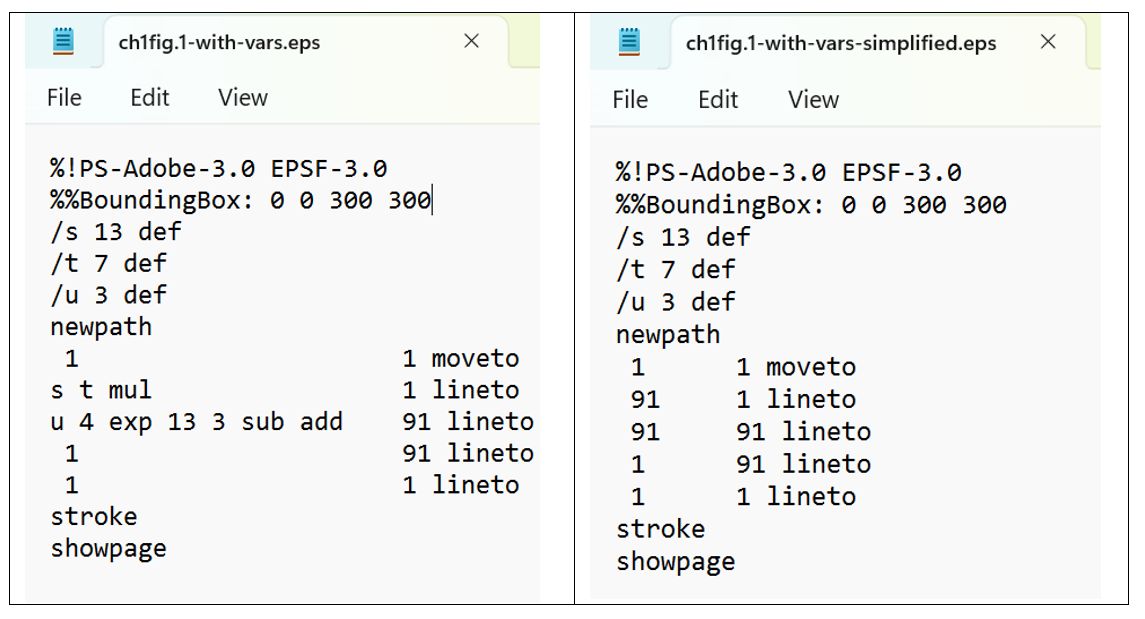
\includegraphics[scale=0.45]{fig/simplifiedFile.png}
	\caption{Original File Vs Simplified File with Variable declaration}
\end{figure}

The following figure gives a procedure definition ``/dir'' with the original file, simplified file and the rendered image. Note that the procedure definition is enclosed in curly brackets (braces).
\begin{figure} [H]
	\centering
	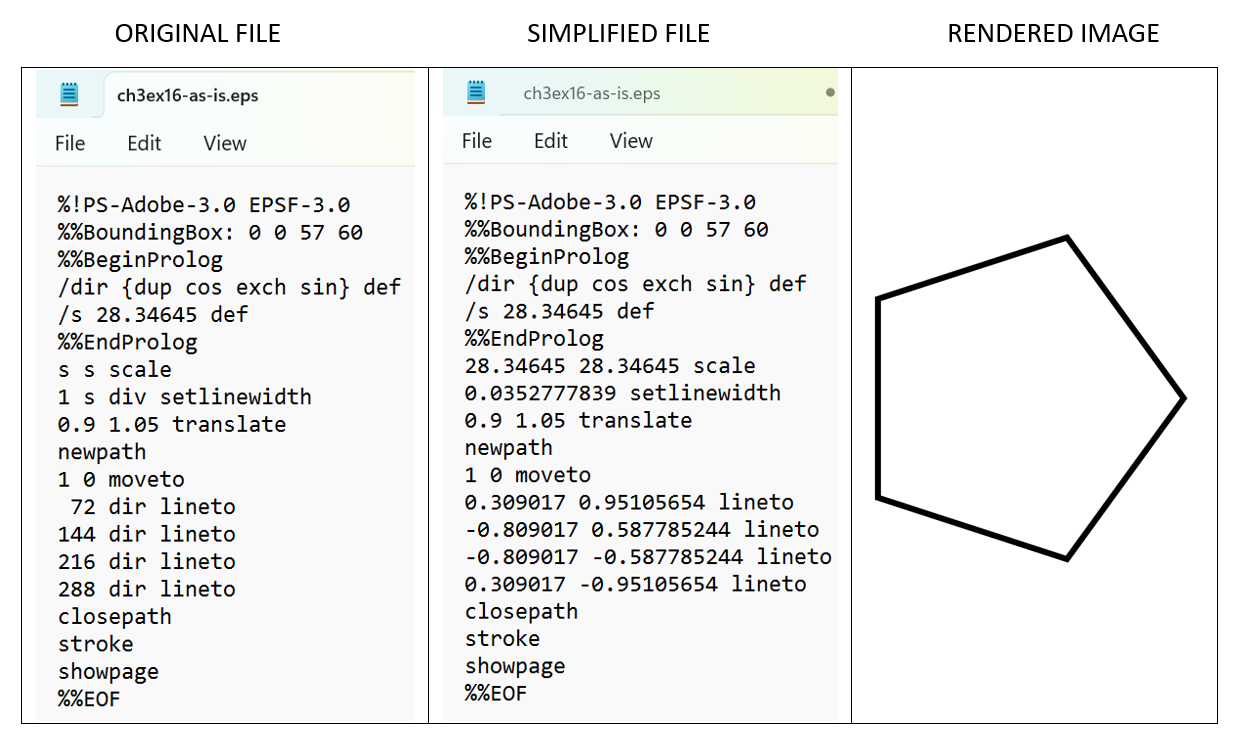
\includegraphics[scale=0.5]{fig/procedureDefinition.png}
	\caption{Original File, Simplified File and And Rendered Image}
\end{figure}
\textbf{Objective:}
Given a postscript file with operations from the tables (Arithmetic and Manipulation Operators), generate a simplified postscript file that does not contain any of the stack based operators – instead it contains the results of evaluations of these operators.

\vspace{0.5cm}

\textbf{Problem Description:} Design and implement a class \texttt{PostScriptFileSimplifier} in C++ that:
\begin{itemize}
\item (5 points) reads in a postscript file into an appropriate data structure of your choice, 
\item (10 points) replaces all variable and procedure names with their simplified definitions in the data structure. This can be achieved by storing and utilizing information about variables and procedures along with the required functions in another data structure, 
\item (20 points) has a function to simplify the postscript file by evaluating all stack based operations and removing these from the actual postscript file. You may declare a class \texttt{StackPostscript} that uses a Stack data structure and implements various stack based operations as shown in Figures 3 and 4,
\item (5 points) writes the simplified postscript file as \texttt{<originalfile>-simplified.ps} (or .eps).
\end{itemize}
\end{homeworkProblem}

We are providing you with two folders: \texttt{input} containing input files and \texttt{output} containing the corresponding simplified output files. Your program should read in every input file in the input folder and produce the corresponding output files in a folder called "test-output".
\\

Further submission guidelines will be provided to you later.
\\

Due date: Saturday, 10 March 2024, 11.59pm.

\end{document}

